\section{Design patterns}
\subsection{Ziel}
\begin{itemize}
	\item Eine elementare Lösung für wiederauftretende Probleme
	\item Die Lösung so präparieren, dass sie in vielen analogen Bereichen eingesetzt werden kann
	\item Als best practice Vorschlag im Software Design dienen   
\end{itemize}
\subsection{Creational Patterns}
\subsubsection{Factory}
Zur Kompilierzeit sollte die erzeugende Klasse nur die Basisiklasse des zu erzeugenden Objekts kennen und nicht deren Subklassen. Die Erzeugung von Objekten wird an Subklassen übergeben mithilfe der factoryMethod(), welche den virtuellen constructor ersetzt.
\begin{table}[H]
\caption{Factory}
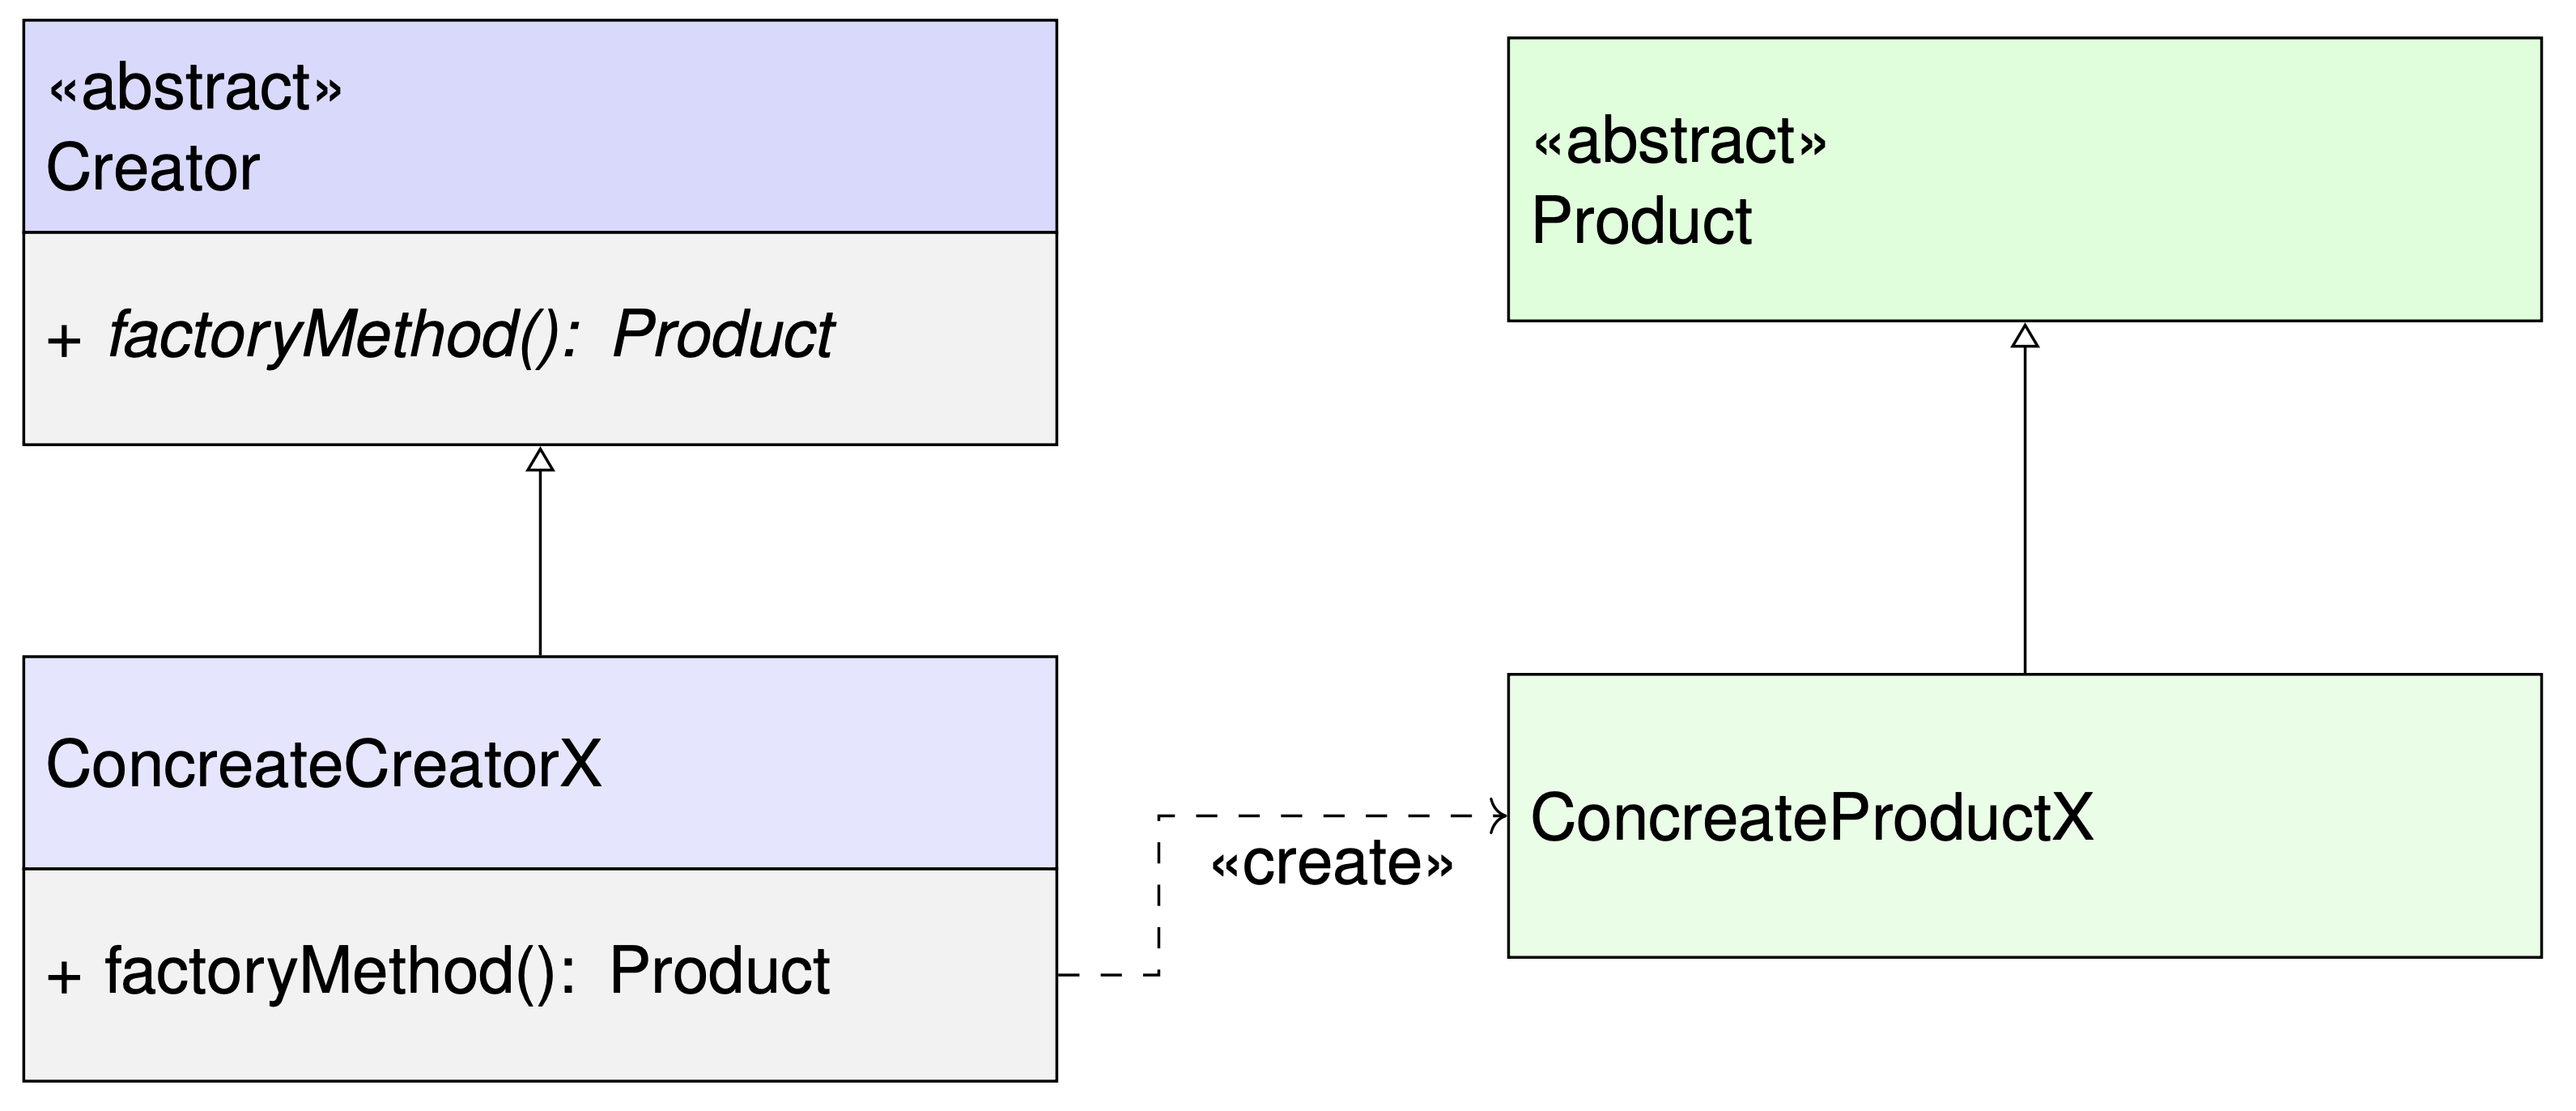
\includegraphics[scale=0.25]{Factory.png}	
\end{table}
\begin{multicols}{2}
$\bold{Pros}$:
\begin{itemize}
	\item Anwendungen müssen nicht die spezifischen Produktklassen kennen
	\item Erzeugungsprozess ist im Creator entkapselt und austauschbar
	\item Verschiedene konkrete Produkte, verschiedener Typen können erzeugt werden  
\end{itemize}
\columnbreak
$\bold{Cons}$:
\begin{itemize}
	\item Erhöhte Komplexität
	\item Geminderte Performance
	\item Konkrete Creators sind stark mit konkreten Produkten verkünpft
\end{itemize}
\end{multicols}
\subsubsection{Abstract Factory}
Bietet ein Interface an, um Familien von verbundenen oder abhängigen Objekten zu erzeugen, ohne konkrete Klassen zu spezifizieren und entscheidet zur Laufzeit, welche Produktfamilie generiert wird, indem die verantwortliche konkrete Factory gewählt wird
\begin{table}[H]
\caption{Abstract factory with client}
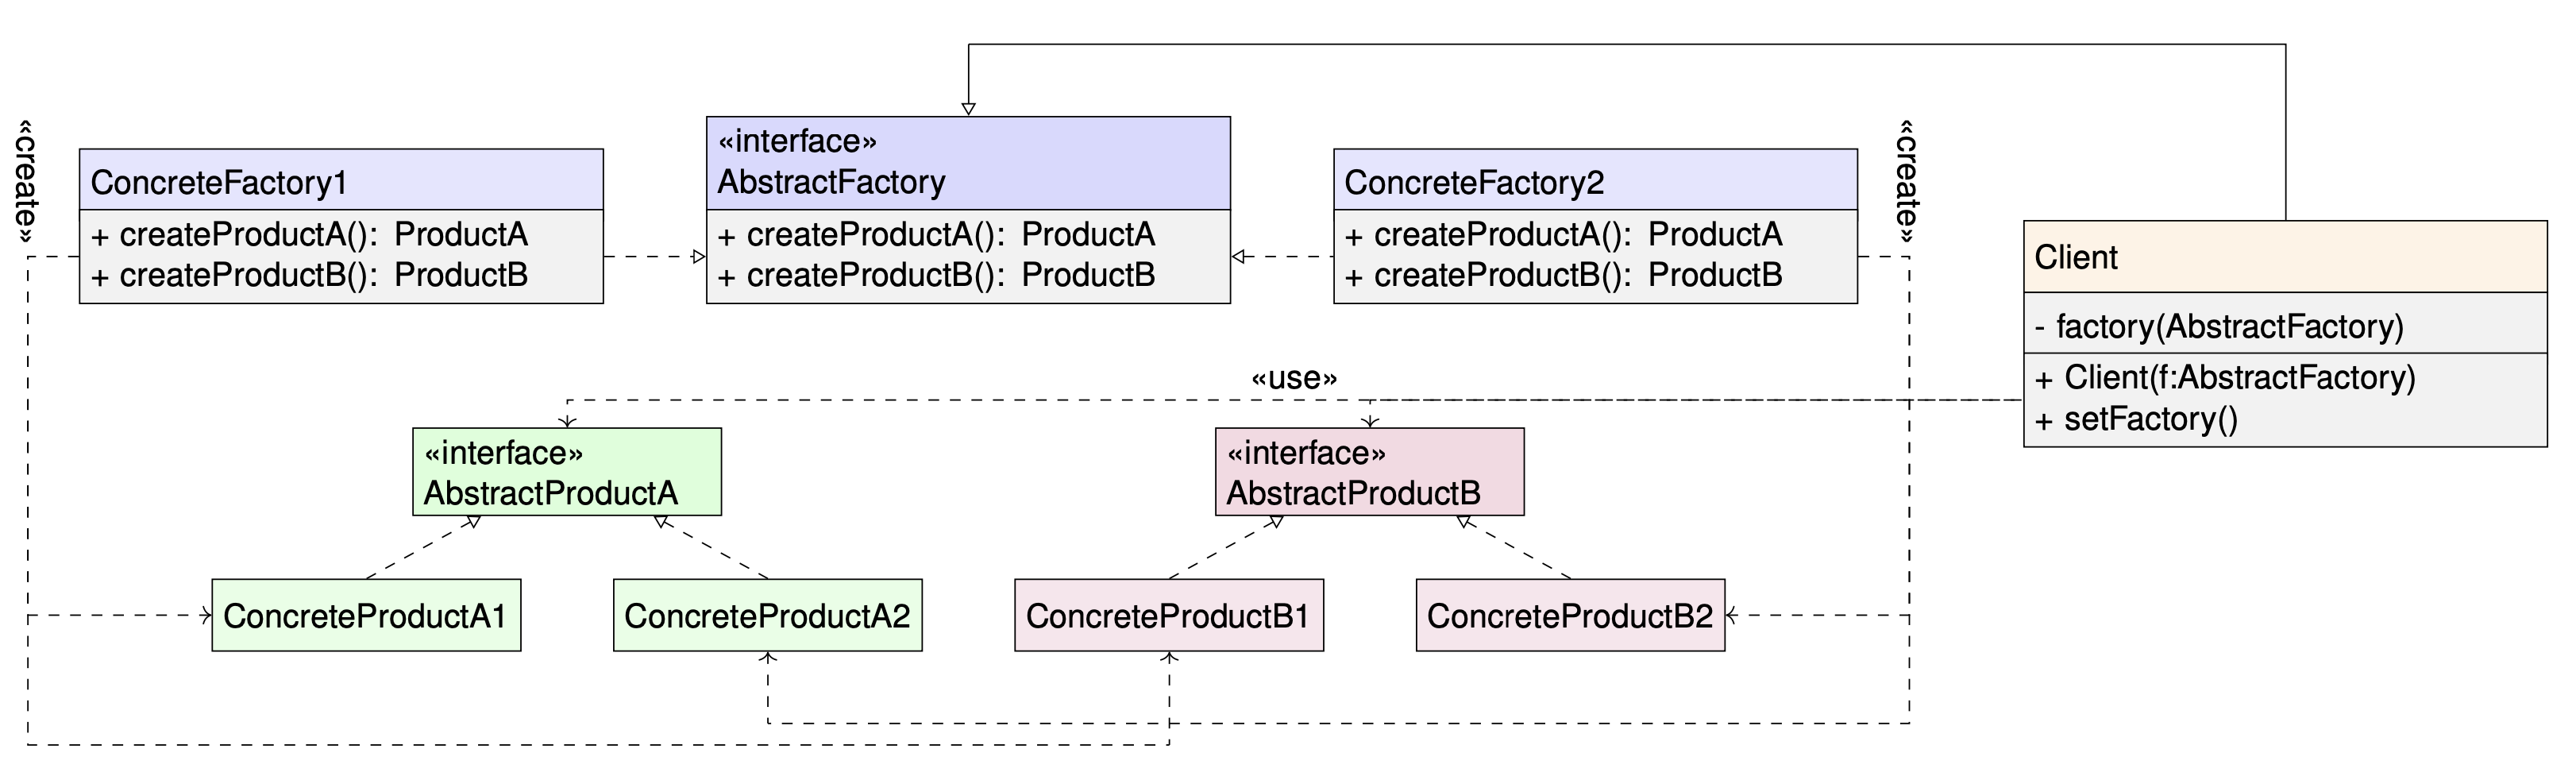
\includegraphics[scale=0.25]{Abstract_factory.png}
\end{table}
\begin{multicols}{2}
$\bold{Pros}$:
\begin{itemize}
	\item Entkopplung der konkrete Implementation durch abstrakte Klassen
	\item Einfaches Austauschen der Porduktfamilien
	\item Konkrete Factories werden erst zur Laufzeit definiert
\end{itemize}
\columnbreak
$\bold{Cons}$:
\begin{itemize}
	\item Erweiterung der Produktfamilie mit neuen Produkttyoen ist teuer
\end{itemize}
\end{multicols}
\subsubsection{Builder}
Den Erzeugungsprozess komplexer Klasse vereinfachen, indem man den Konstruktionsprozess in eine spezielle Klasse zieht
\begin{table}[H]
\caption{Builder}
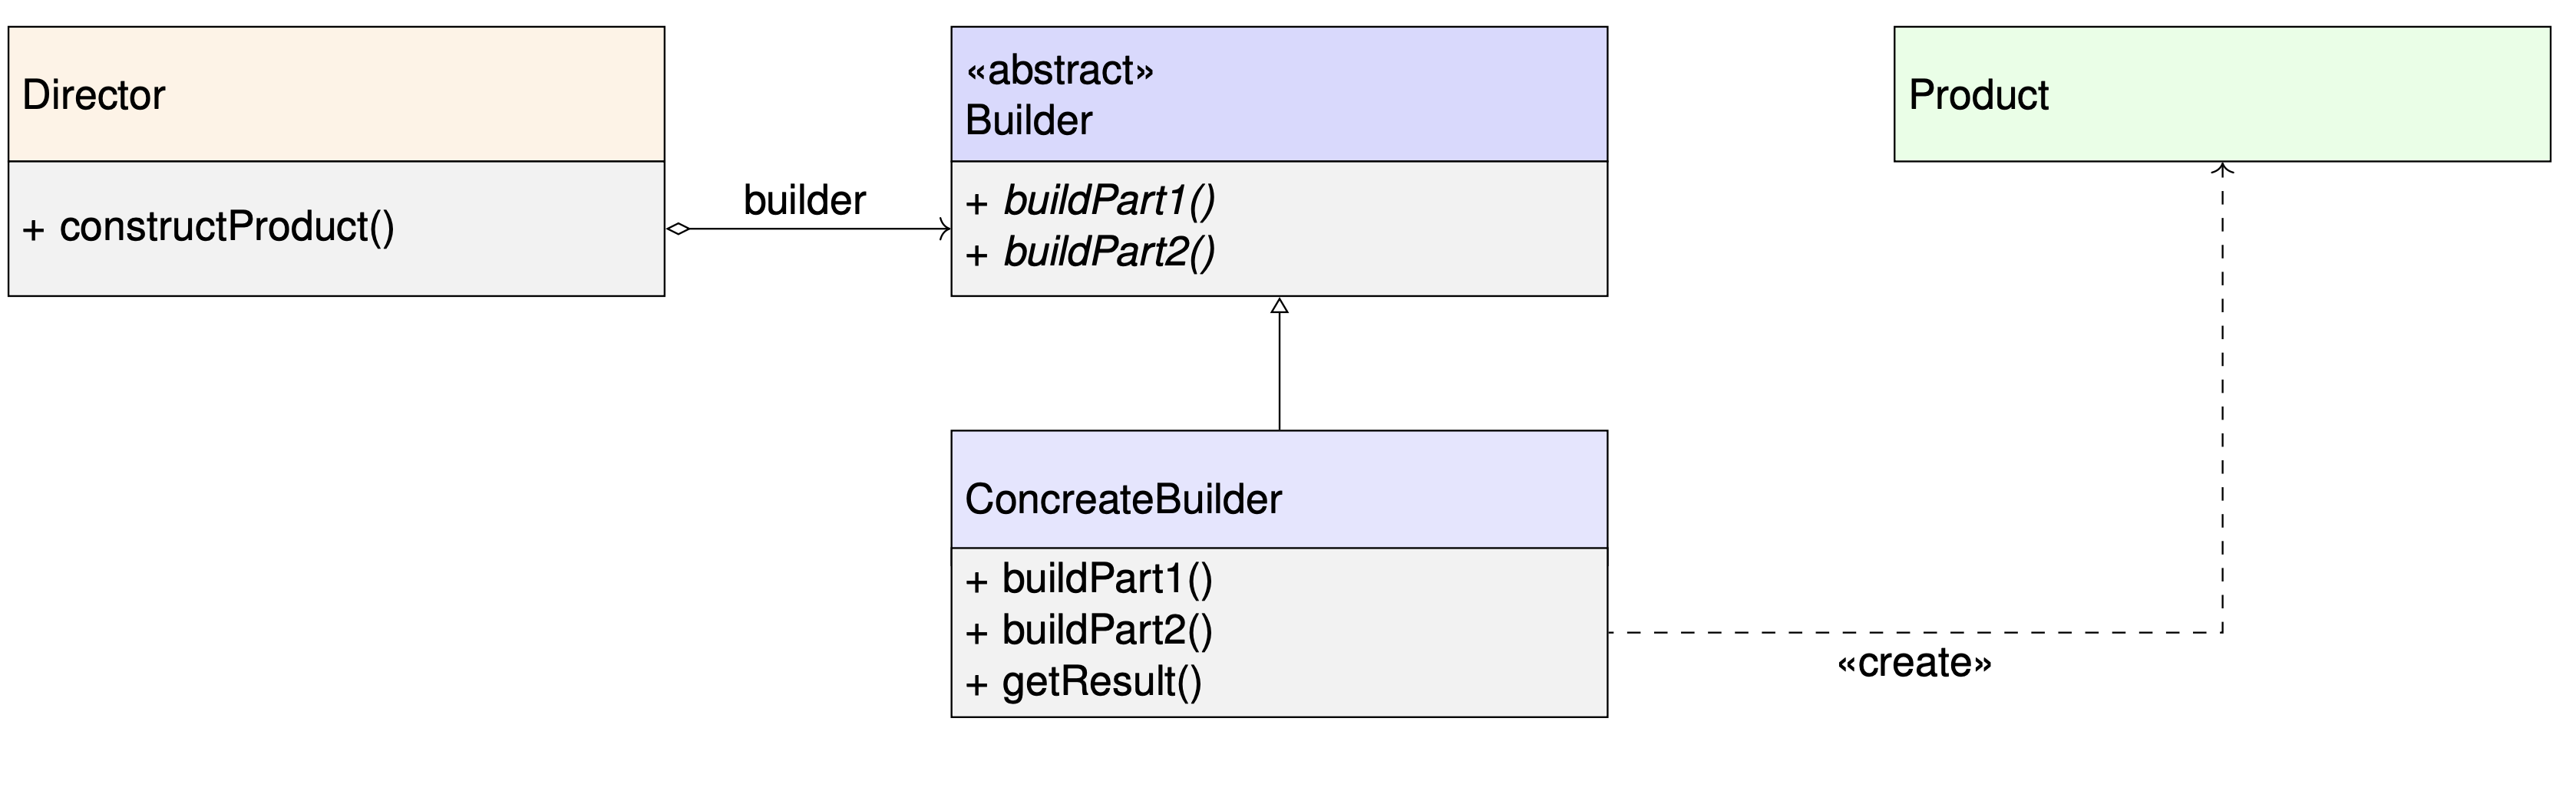
\includegraphics[scale=0.25]{builder.png}
\end{table}
\begin{multicols}{2}
$\bold{Pros}$:
\begin{itemize}
	\item Die Implementierung der Konstruktion und deren Repräsentation sind isoliert
	\item Besser erweiterbar und erhaltbar
	\item Neue konkrete Builder können einfach integriert werden
	\item Die Directorklasse verbirgt die Details der Konstruktion vom Client 
\end{itemize}	
\columnbreak
$\bold{Cons}$:
\begin{itemize}
	\item Produkt und konkreter Builder sind stark verbunden
	\item Für jede neue Repräsentation muss ein neuer konkreter Builder erzeugt werden
\end{itemize}
\end{multicols}
\subsubsection{Prototyp}
Kopieren der existierenden Objekte, ohne den Code von deren Klassen abhängig zu machen. Die konkreten Prototypen implementieren eine cloningMethod(), welche das Objekt erzeugen und alle Felder kopieren
\begin{table}[H]
\caption{Prototyp}
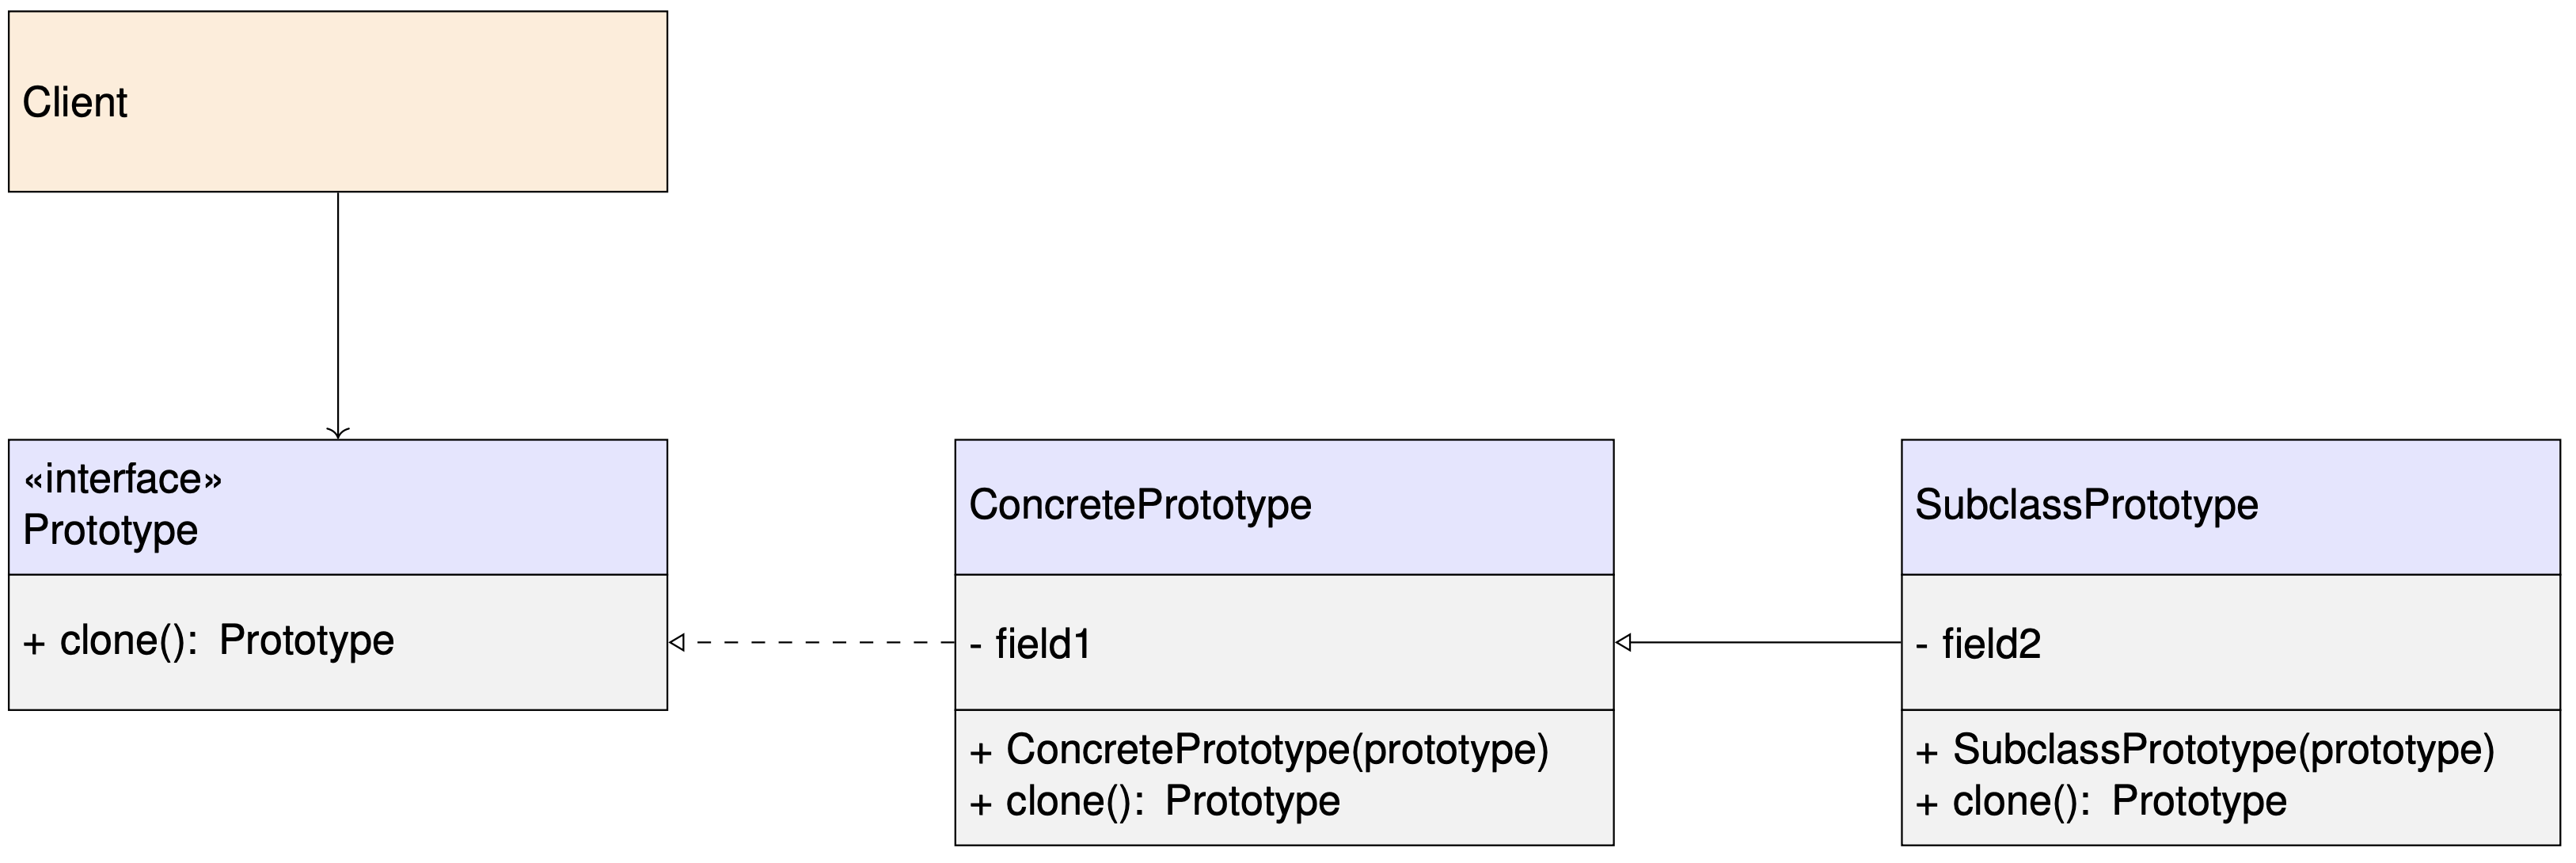
\includegraphics[scale=0.25]{Prototyp.png}	
\end{table}
\begin{multicols}{2}
$\bold{Pros}$:
\begin{itemize}
	\item Klone Objekte ohne Verknüpfung zu der konkreten Klasse
	\item Kein wiederholter Initialisierungscode 
	\item Kann eine alternative zu Vererbung sein  
\end{itemize}
\columnbreak	
$\bold{Cons}$:
\begin{itemize}
	\item Komplexe Objekte zu klonen kann schwer sein
\end{itemize}
\end{multicols}
\subsubsection{Singelton}
Durch ausschließliche Erzeugung mit der Singletonklasse wird es möglich, dass eine Klasse nur einmal initialisiert wird 
\begin{table}[H]
\caption{Singleton}
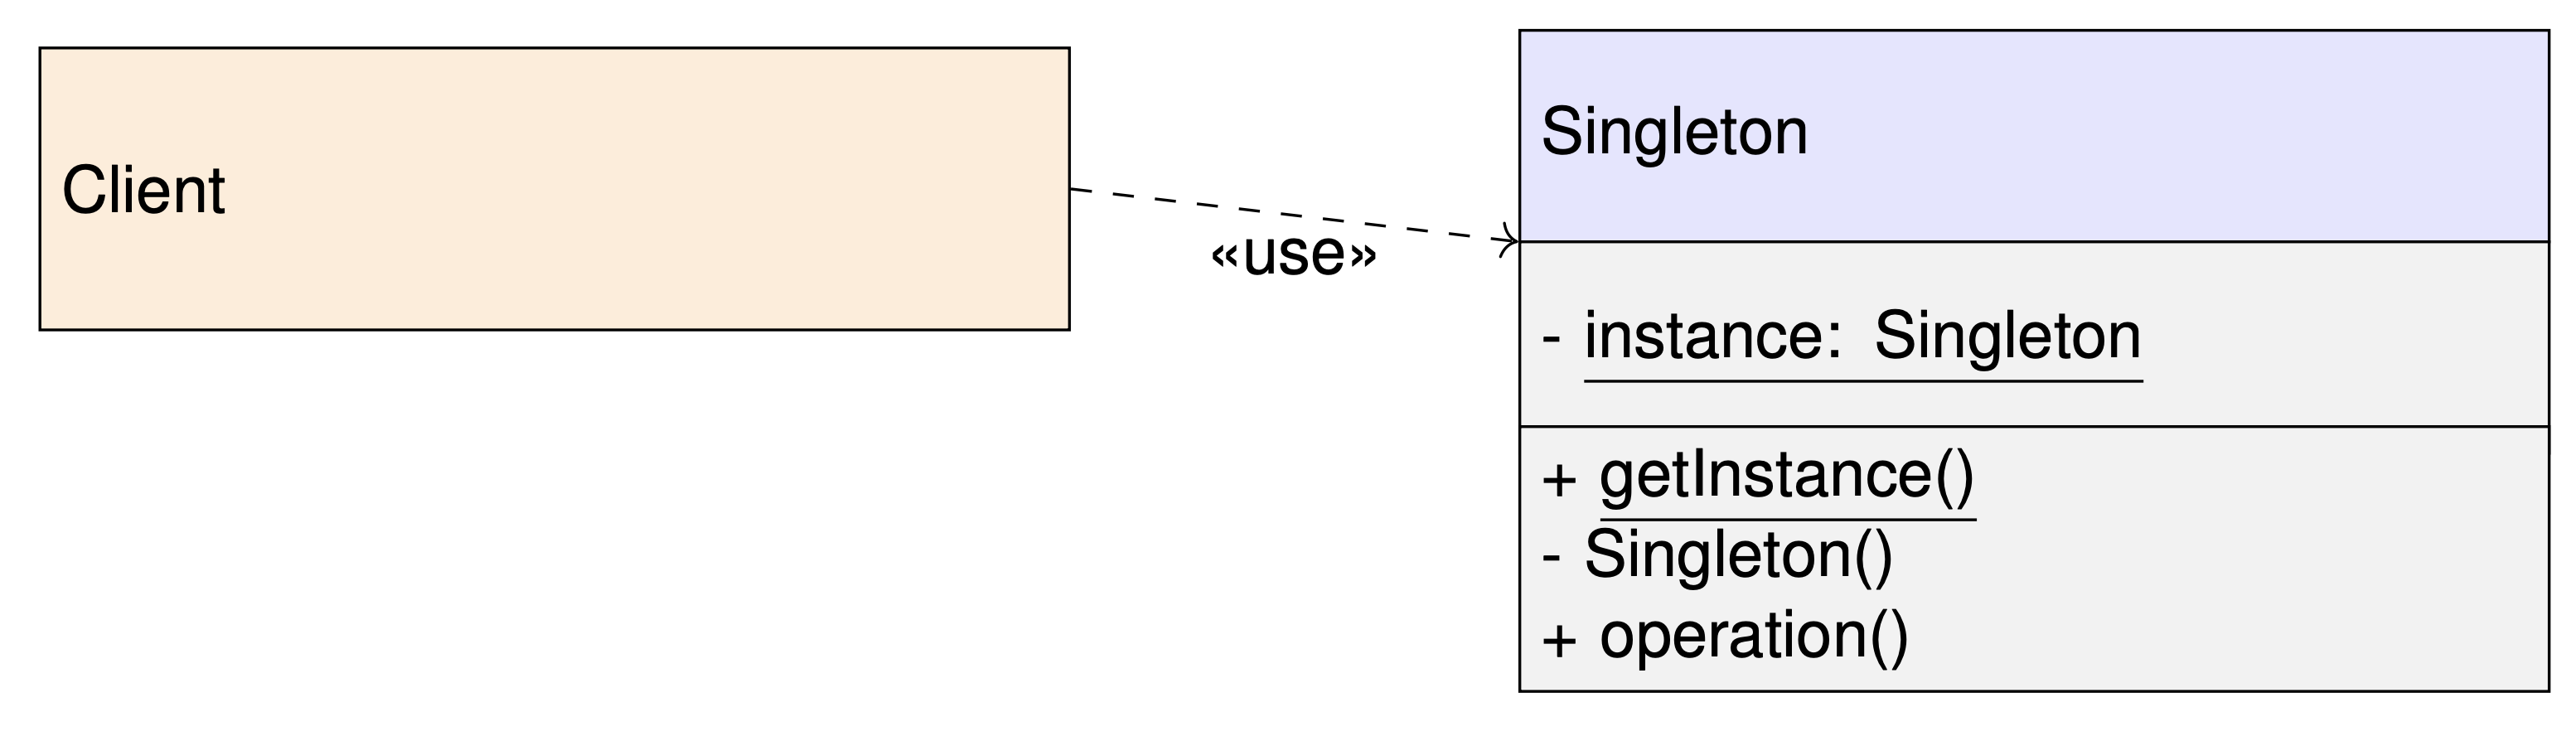
\includegraphics[scale=0.25]{Singleton.png}	
\end{table}
\begin{multicols}{2}
$\bold{Pros}$:
\begin{itemize}
	\item Nur ein Single wird erzeugt
	\item Erhalte einen globalen Zugriffspunkt zu dieser Instanz
\end{itemize}
\columnbreak
$\bold{Cons}$:
\begin{itemize}
	\item Schwer bei verteilten oder multi-threaded Anwendungen
\end{itemize}
\end{multicols}
\subsection{Structural Patterns}
Strukturpatterns beschreiben den Weg, wie Klassen oder Objekte zu einer größeren Struktur kombiniert werden können  
\subsubsection{Adapter}
Um Klassen weiterzuverwenden, die das falsche Interface für die neue Anwendung haben werden Adapter als Übersetzungsschicht eingesetzt. Ein Klassenadapter kann nur auf eine Klasse aufsetzen, ein Objektadapter kann auch auf deren Subklassen aufsetzten
\begin{table}[H]
\caption{Class adapter}
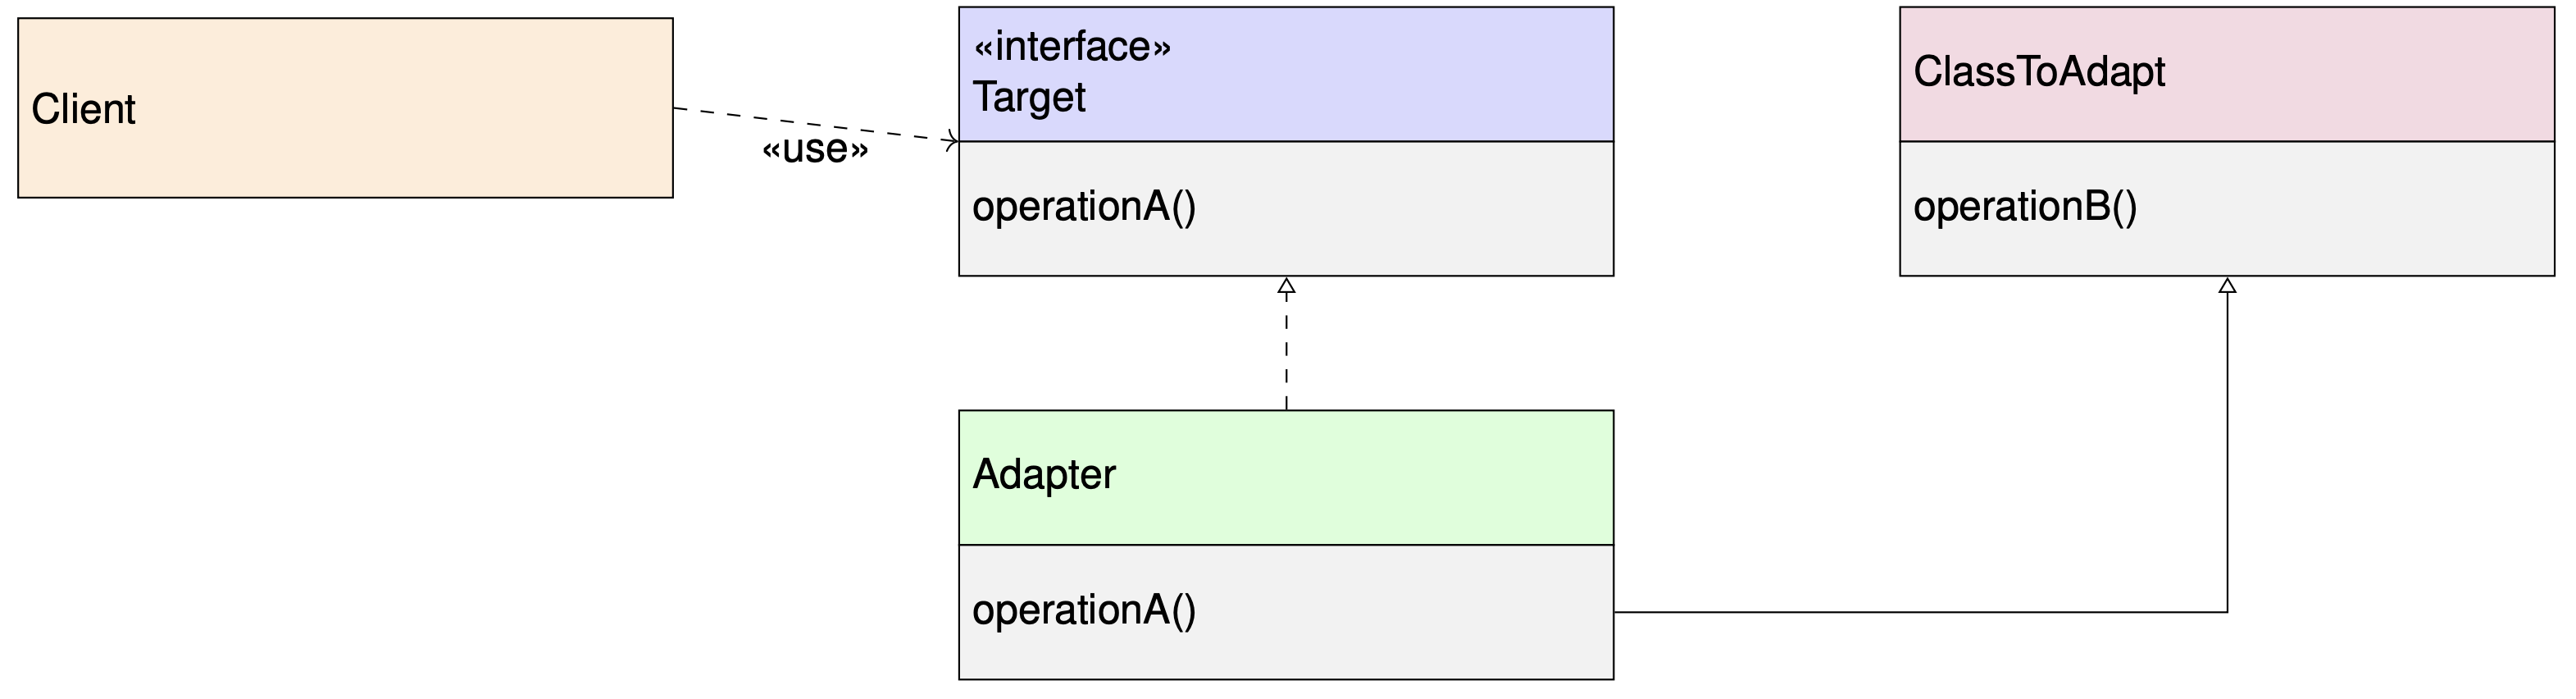
\includegraphics[scale=0.25]{Class_adapter.png}	
\end{table}
\begin{table}[H]
\caption{Object adapter}
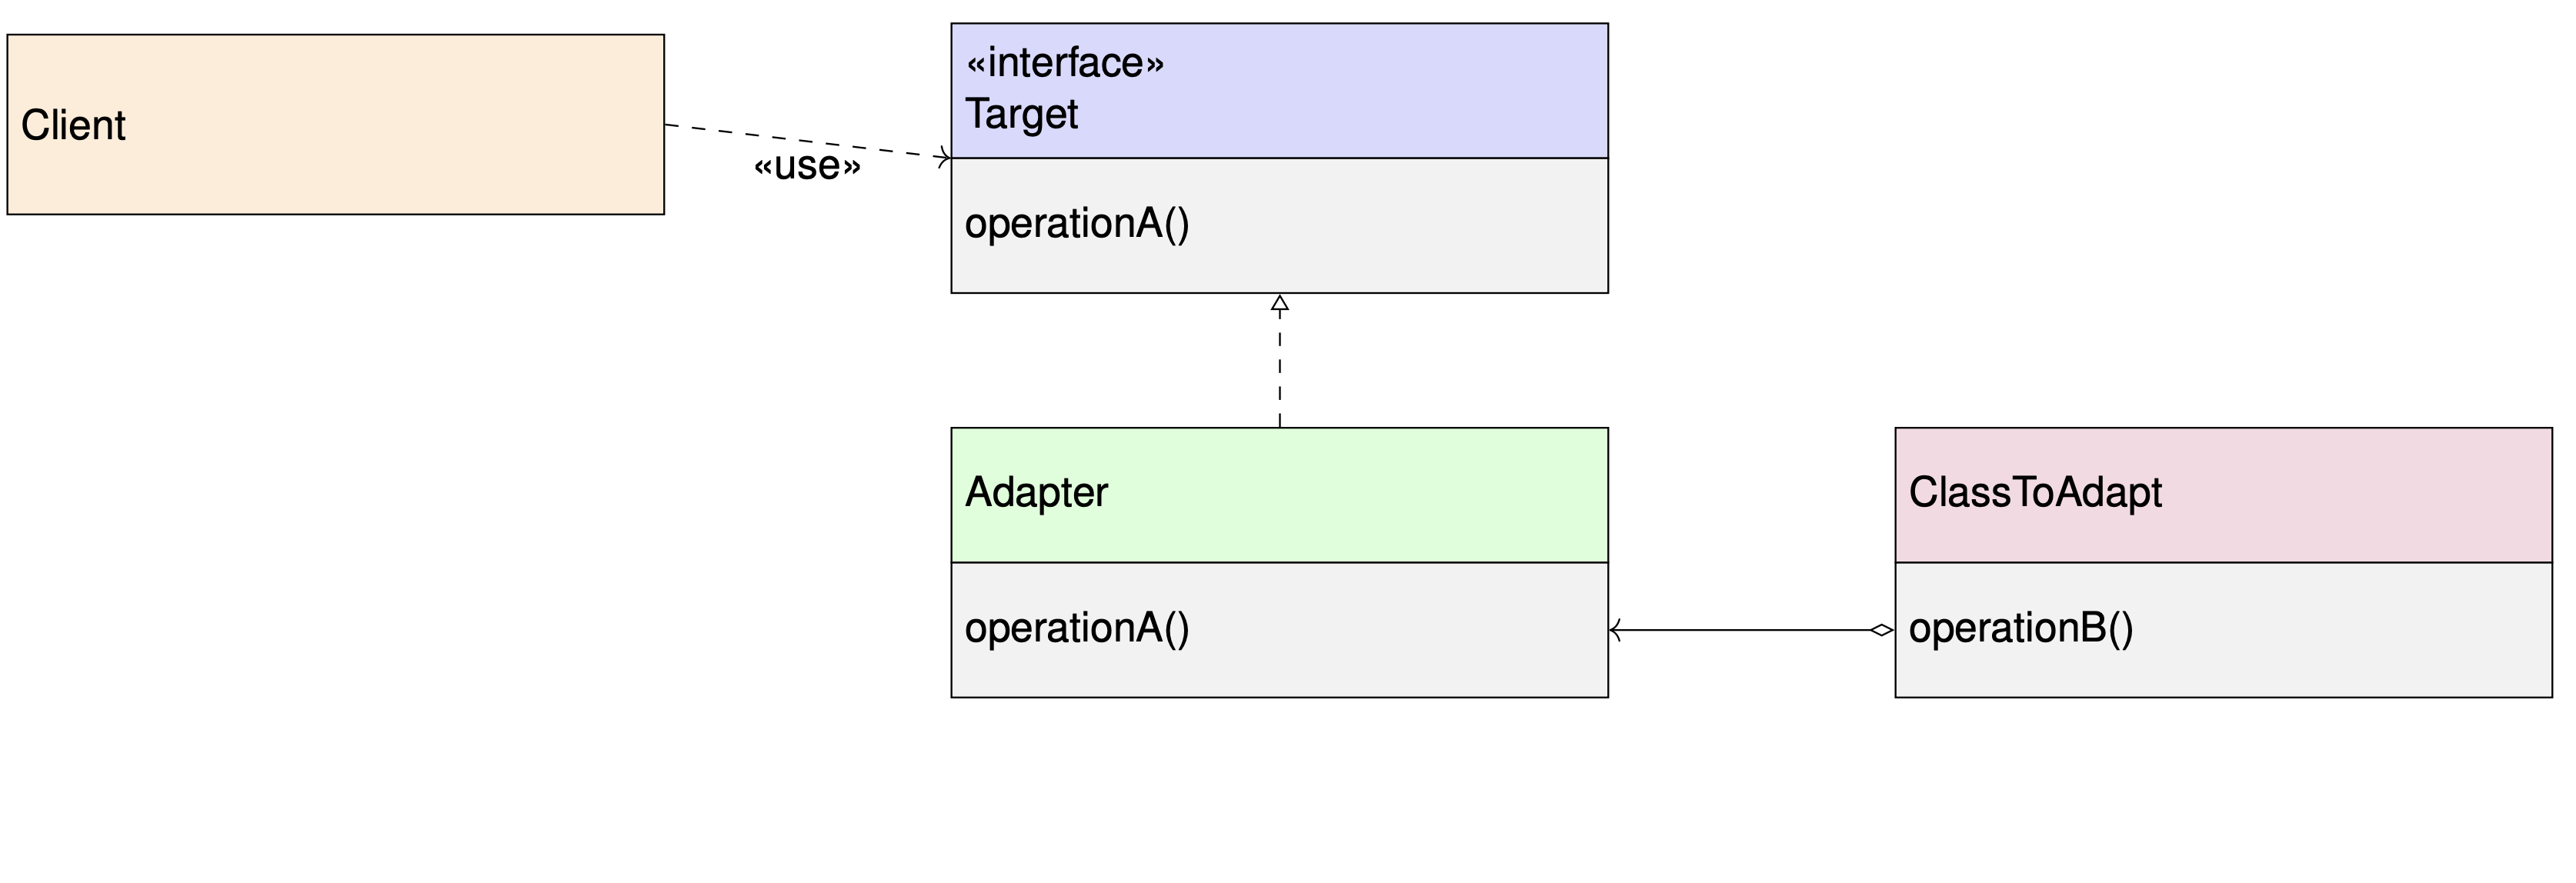
\includegraphics[scale=0.25]{Object_adapter.png}	
\end{table}
\begin{multicols}{2}
$\bold{Pros}$:
\begin{itemize}
	\item Kommunikation zwischen zwei unabhängigen Komponenten 
\end{itemize}
\columnbreak
$\bold{Cons}$:
\begin{itemize}
	\item Kann zu Zeitverzögerung führen
	\item Limitierte Wiederverwedbarkeit 
	\item Klassenadapter können nicht für Subklassen verwendet werden
	\item Programmiersprache muss Interfaces oder Mehrfachvererbung unterstützen
\end{itemize}
\end{multicols}
\subsubsection{Bridge}
\begin{table}[H]
\caption{Bridge}
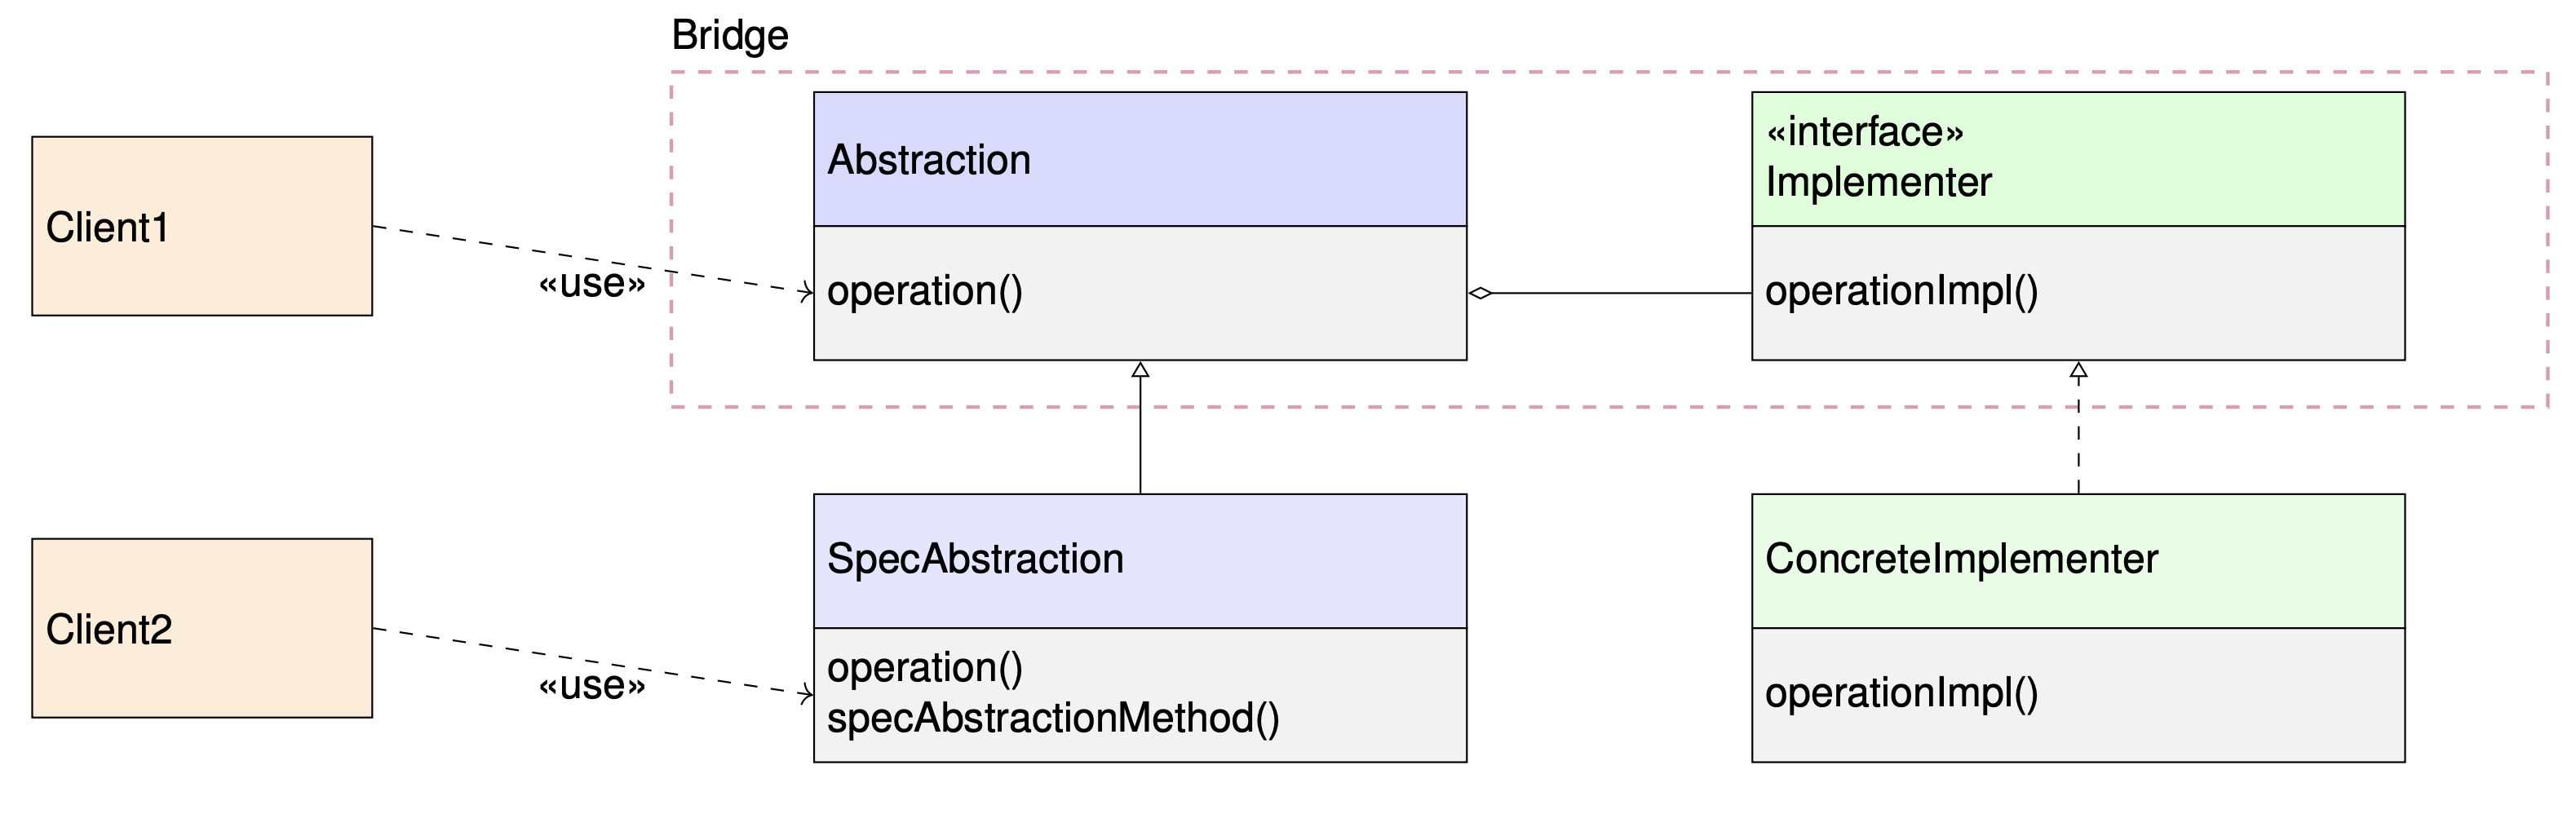
\includegraphics[scale=0.25]{Bridge.png}	
\end{table}
\begin{multicols}{2}
$\bold{Pros}$:
\begin{itemize}
	\item Implementation ist vorm Client verborgen
	\item Unabhängigkeit der Abstraktion und der konkreten Implementation
	\item Beides, Abstraktion und Implementation können unabhängig von einander Subklassen haben
	\item Dynamische Modifikationen, da die Zuweisung einer Implementation während der Laufzeit geschehen kann
	\item Geteilte Nutzung von Implementationen für verschiedene Abstraktionen  
\end{itemize}	
\columnbreak
$\bold{Cons}$:
\begin{itemize}
	\item Schwer einen Überblick zu erlangen, wegen der vielen Klassen
\end{itemize}
\end{multicols}
\subsubsection{Decorator}
Erweitert die Funktionalität eines Objekts zur Laufzeit
\begin{table}[H]
\caption{Decorator}
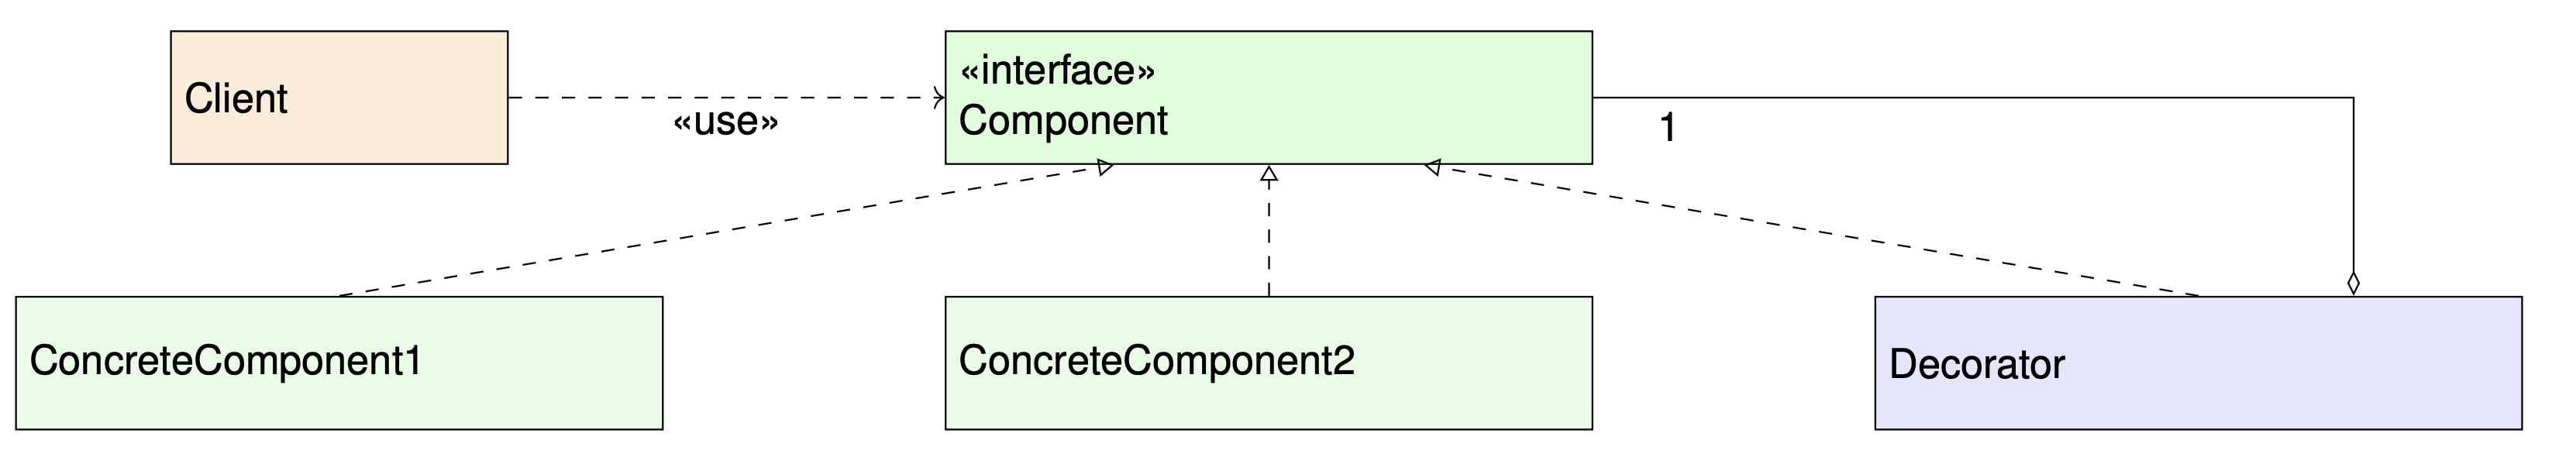
\includegraphics[scale=0.25]{Decorator.png}	
\end{table}
\begin{multicols}{2}
$\bold{Pros}$:
\begin{itemize}
	\item Nutzt Aggregation anstatt Vererbung, um zusätzliche Funktionalität zu bieten
	\item Komponenten kennen ihren Decorator nicht
	\item Gleichzeitige Dekoration von verschiedenen Klassen
	\item Kombination mehrerer Decorators
\end{itemize}	
\columnbreak
$\bold{Cons}$:
\begin{itemize}
	\item Hohe Anzahl an Decorators führt zu hoher Anzahl an ähnlichen Klassen
	\item Verzögerung durch Delegation
	\item Schwer zu implementieren, sodass der Decorator unabhängig ist 
\end{itemize}
\end{multicols}
\subsubsection{Facade}
Präsentiert ein Subsystem, als wäre es ein Objekt mit Interface
\begin{table}[H]
\caption{Facade}
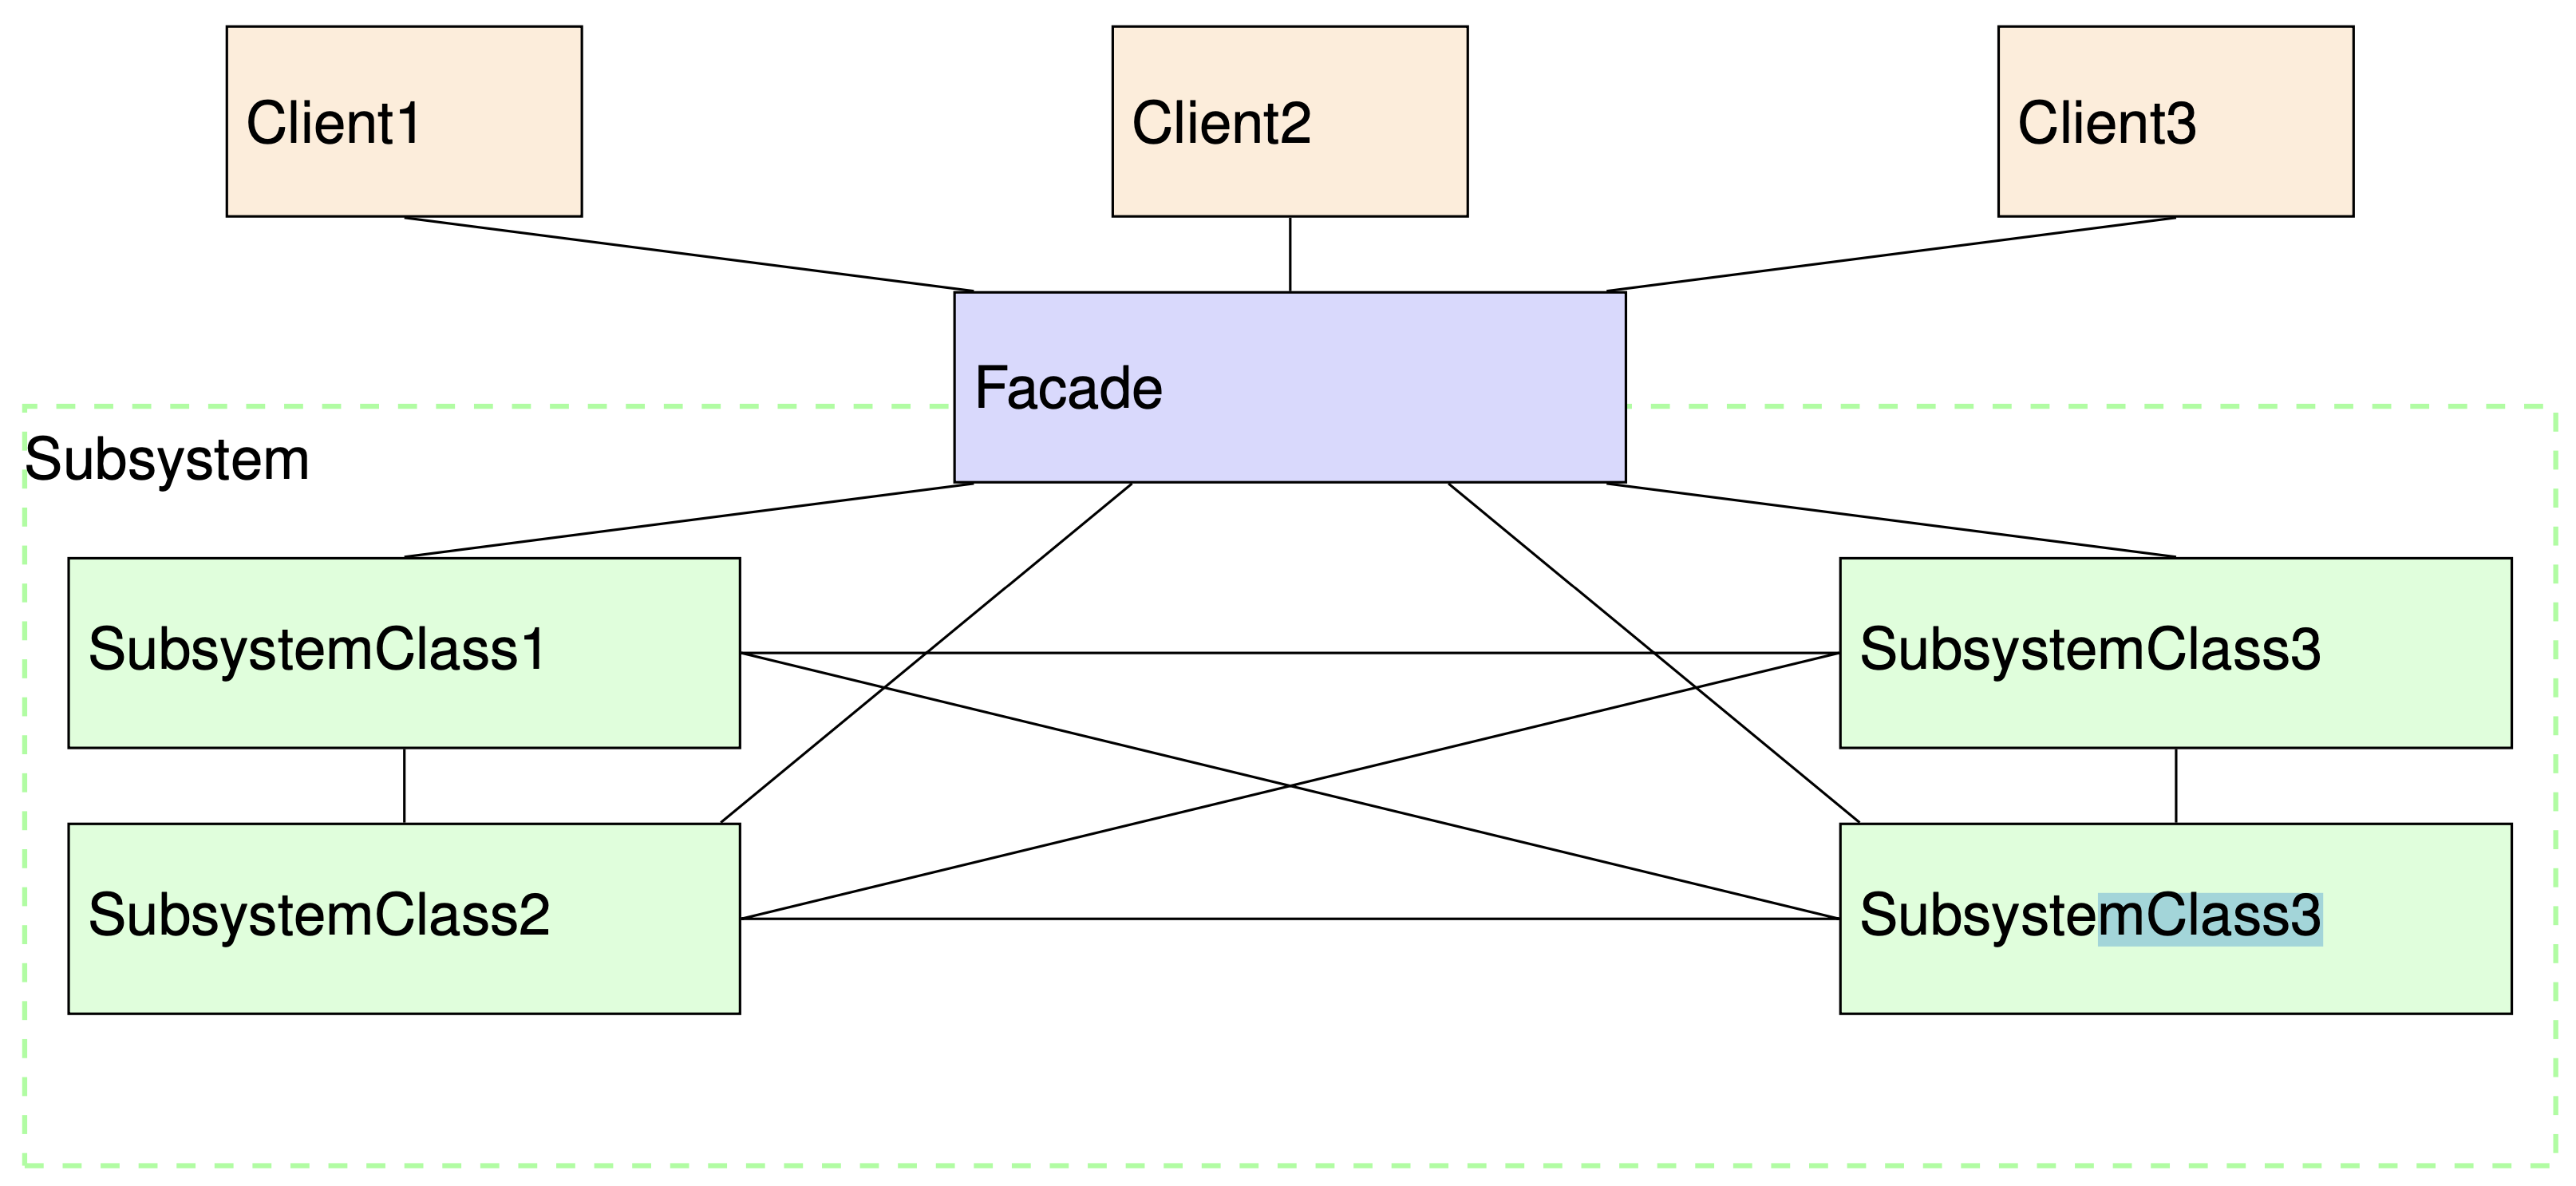
\includegraphics[scale=0.25]{Facade.png}
\end{table}
\begin{multicols}{2}
$\bold{Pros}$:
\begin{itemize}
	\item Entkoppelt Client und Details des Subsystems
	\item Implementation und Interface des Subsystems können geändert werden, ohne Veränderungen beim Client 
\end{itemize}
\columnbreak
$\bold{Cons}$:
\begin{itemize}
	\item Client könnte einen Weg finden, die Facade zu umgehen
	\item Implementation der Facade müsste angepasst werden, wenn die Interfaces des Subsystems sich verändern
\end{itemize}
\end{multicols}
\subsubsection{Composite}
Verarbeitet Objekte in einer Baumstruktur
\begin{table}[H]
\caption{Composite}
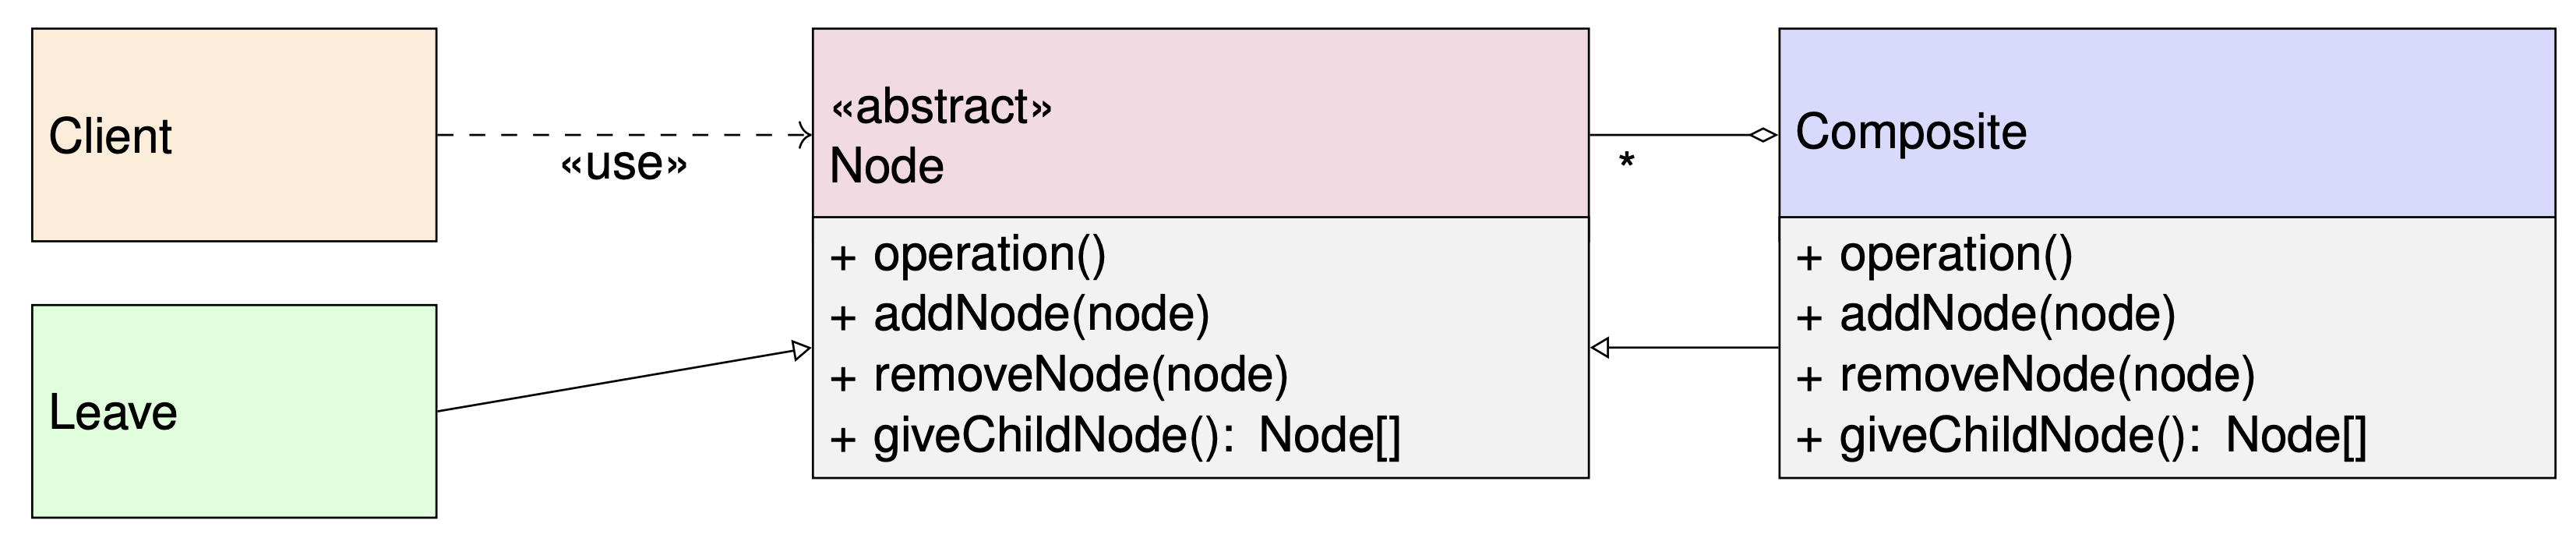
\includegraphics[scale=0.25]{Composit.png}
\end{table}
\begin{multicols}{2}
$\bold{Pro}$:
\begin{itemize}
	\item Einfachere Implementation des Client-Zugriffs
	\item Erleichterte Erzeugung verschachtelter Objekte
\end{itemize}	
\columnbreak
$\bold{Cons}$:
\begin{itemize}
	\item Schwer bei Restriktionen
	\item Veränderungen am Node führt zu Veränderungen an den erbenden Klassen
	\item Benennung des allgemeinen Interfaces kann schwer sein 
\end{itemize}
\end{multicols}
\subsubsection{Proxy}
Klasse mit gleichem Interface, wie Implementation. Clients greifen über Proxy auf Implementation zu.
\begin{table}[H]
\caption{Proxy}
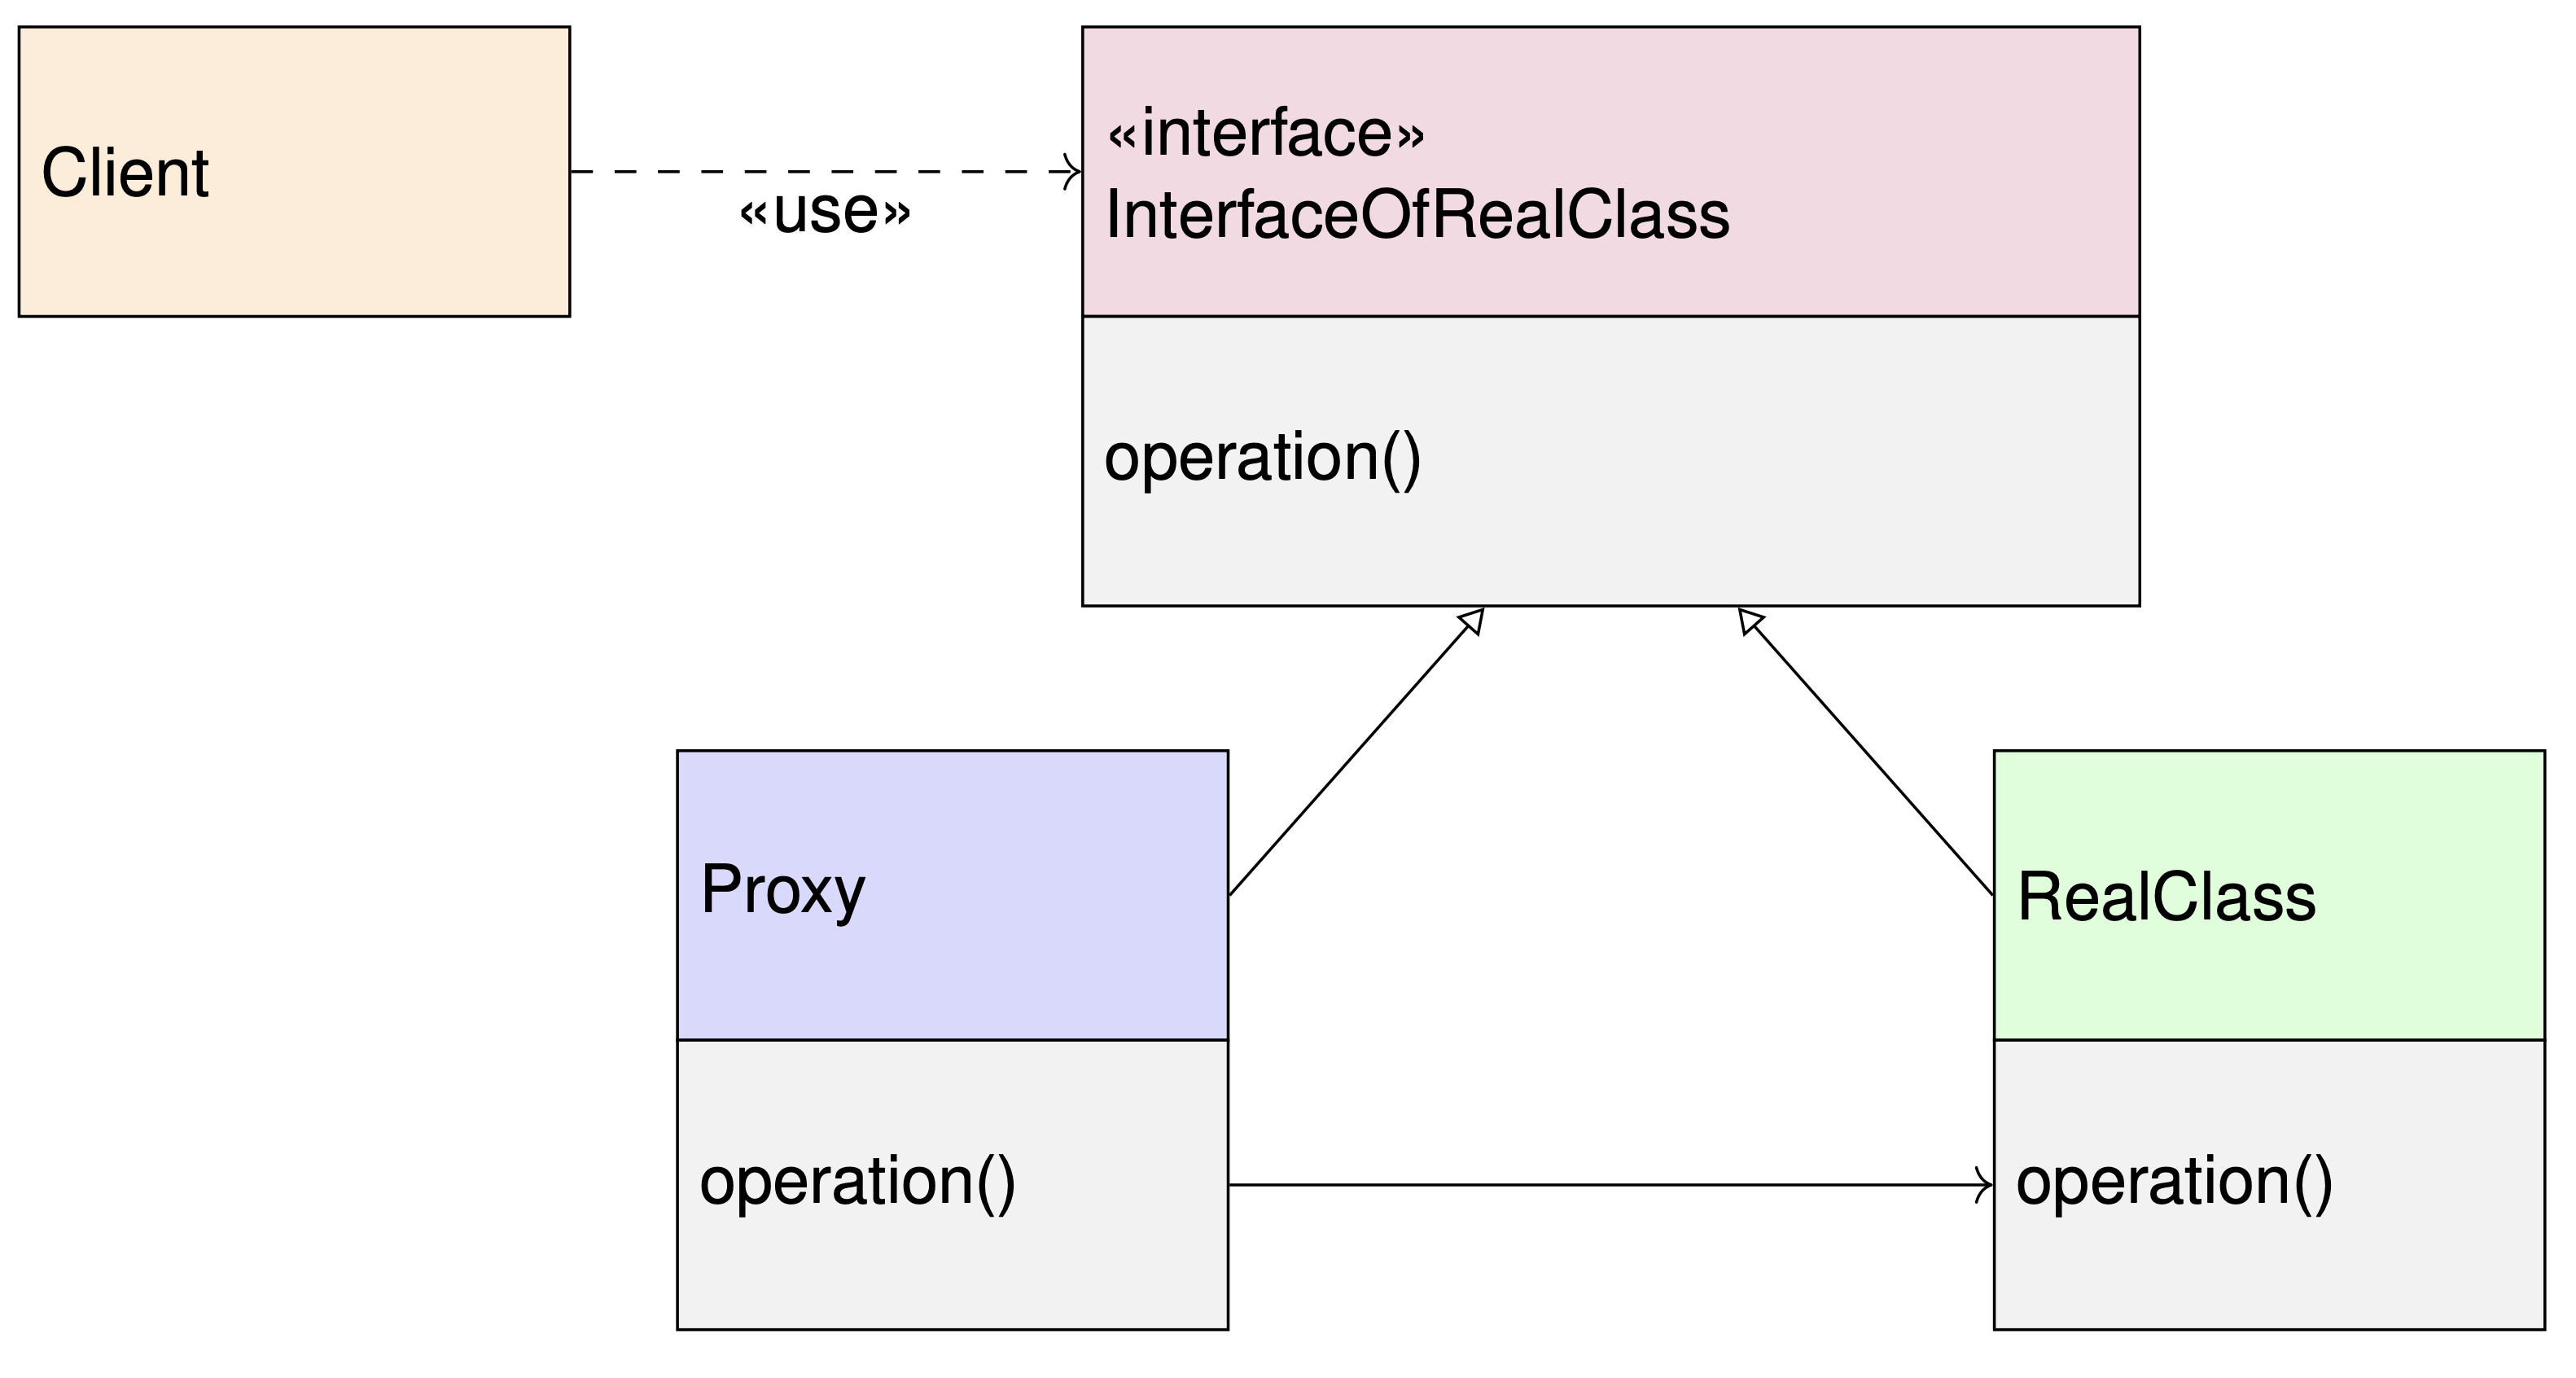
\includegraphics[scale=0.25]{Proxy.png}	
\end{table}
\begin{multicols}{2}
$\bold{Pros}$:
\begin{itemize}
	\item Erweiterung eines existierende Systems
	\item Client braucht nur das allgemeine Interface und kann echtes Objekt nicht von Proxy unterscheiden
	\item Bessere Performance für Operationen, die das echte Objekt nicht brauchen
\end{itemize}
\columnbreak
$\bold{Cons}$:
\begin{itemize}
	\item Macht Fehlerbehebung schwieriger
	\item Performanceverlust, wenn auf echtes Objekt zugegriffen werden muss
	\item Jede Methode muss auch im Proxy implementiert werden
\end{itemize}
\end{multicols}
\subsubsection{Flyweight}
Instanzen werden geteilt, da die Factory maximal eine getielte Instanz jedes Objekts administriert. \newline
Intrinsic state: unabhängig vom Kontext, unantastbar, wird einmal initialisiert \newline
Extrinsic state: abhängig vom Kontext
\begin{table}[H]
\caption{Flyweight}
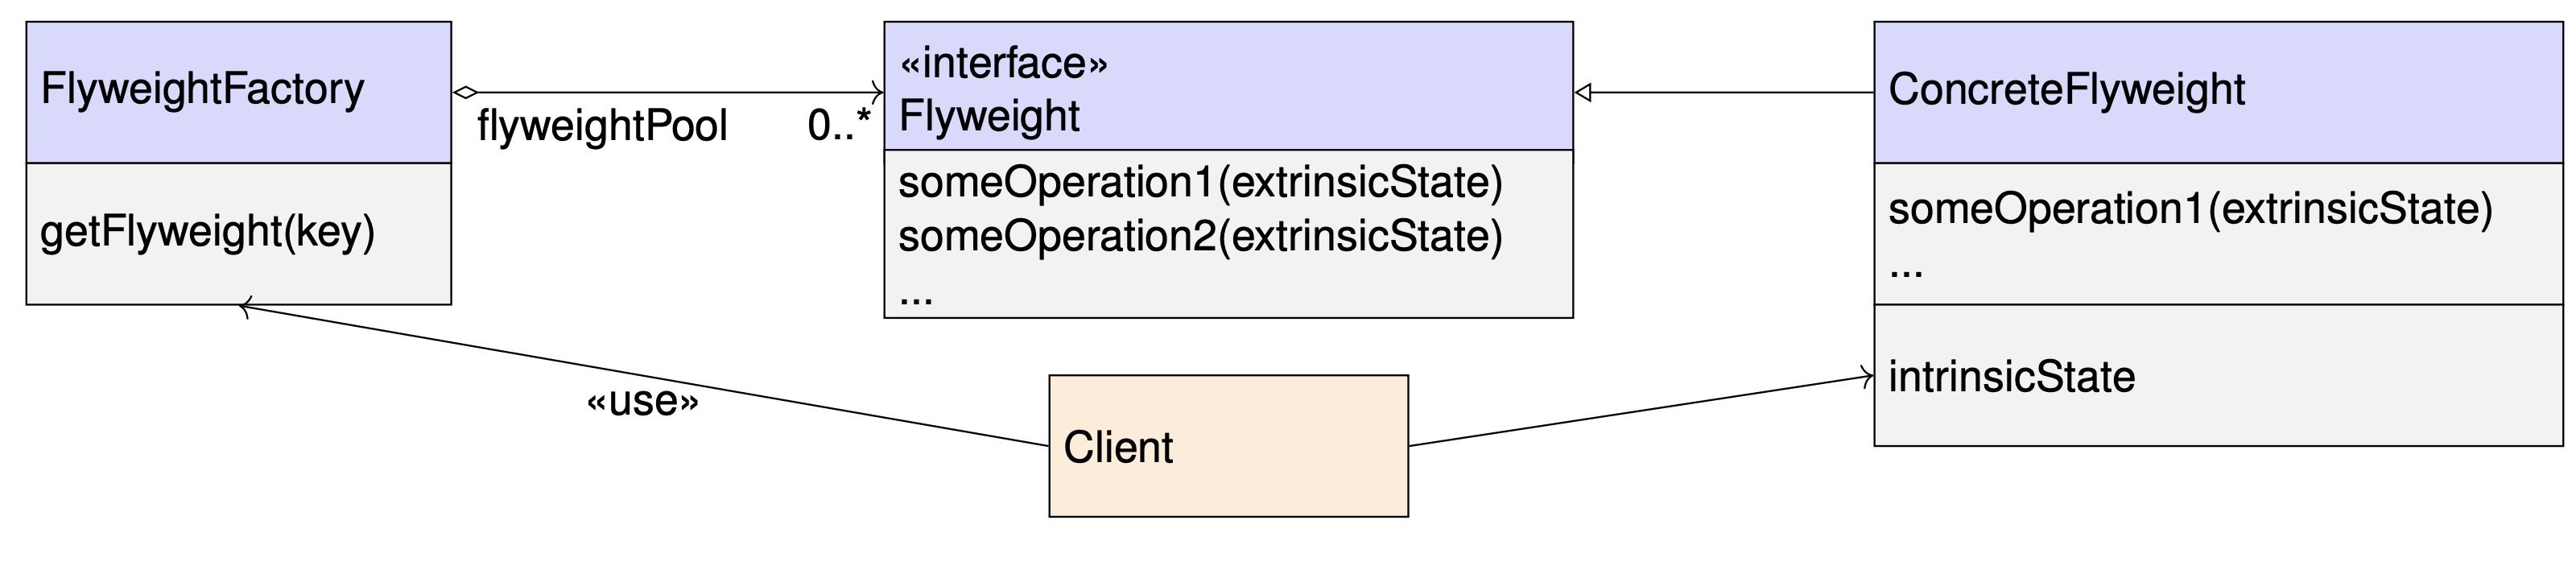
\includegraphics[scale=0.25]{Flyweight.png}	
\end{table}
\begin{multicols}{2}
$\bold{Pros}$:
\begin{itemize}
	\item Reduziert Anzahl an Objektinstanzen, die benötigt werden
	\item Reduktion der Speicheranforderungen
	\item Keine Laufzeitumgebung oder kein Garbage Collector nötig
\end{itemize}
\columnbreak
$\bold{Cons}$:
\begin{itemize}
	\item Berechnen des extrinsic states, des Clients kostet Rechenzeit
	\item Code ist komlpexer
\end{itemize}
\end{multicols}
\subsection{Behavioural Patterns}














